%%%%%%%%%%%%%%%%%%%%%%%%%%%%%%%%%%%%%%%%%%%%%%%%%%%%%%%%%%%%%%%%%%%%%%%%%%%%%%%%
%						FROM SCA TO EVALUATIONS								   %
%%%%%%%%%%%%%%%%%%%%%%%%%%%%%%%%%%%%%%%%%%%%%%%%%%%%%%%%%%%%%%%%%%%%%%%%%%%%%%%%
\subsection{Goals and Stakeholders of the Evaluation and the Certification}

The emergence of side-channel attacks as pervasive and credible threats on modern crypto-systems has contributed to the trend from the industrial and institutional stakeholders of assessing and mitigating them, in order to still ensure the reliability on the security of such crypto-systems.
This is concretely materialized by the emergence of \emph{certification} schemes.
This is a -- sequence of -- process(es) that aim at ensuring that the security claims of a given \gls{toe} are indeed verified, up to the point that a \emph{certification body} can endorse those claims by delivering a security certification.
% Dicsussion about the scope of the TOE
The certification scope depends on the levels of the security, and on the scope of the \gls{toe}: the latter one can either englobe a whole product -- \eg{} a smart card -- or only a specific part of it -- \eg{} its \gls{ic}.
Likewise, the certification is delivered for a given period (\eg{} 3 years), during which it can still be revised depending on the emergence of new threats compromising the security claims.

\begin{figure}
	\centering
	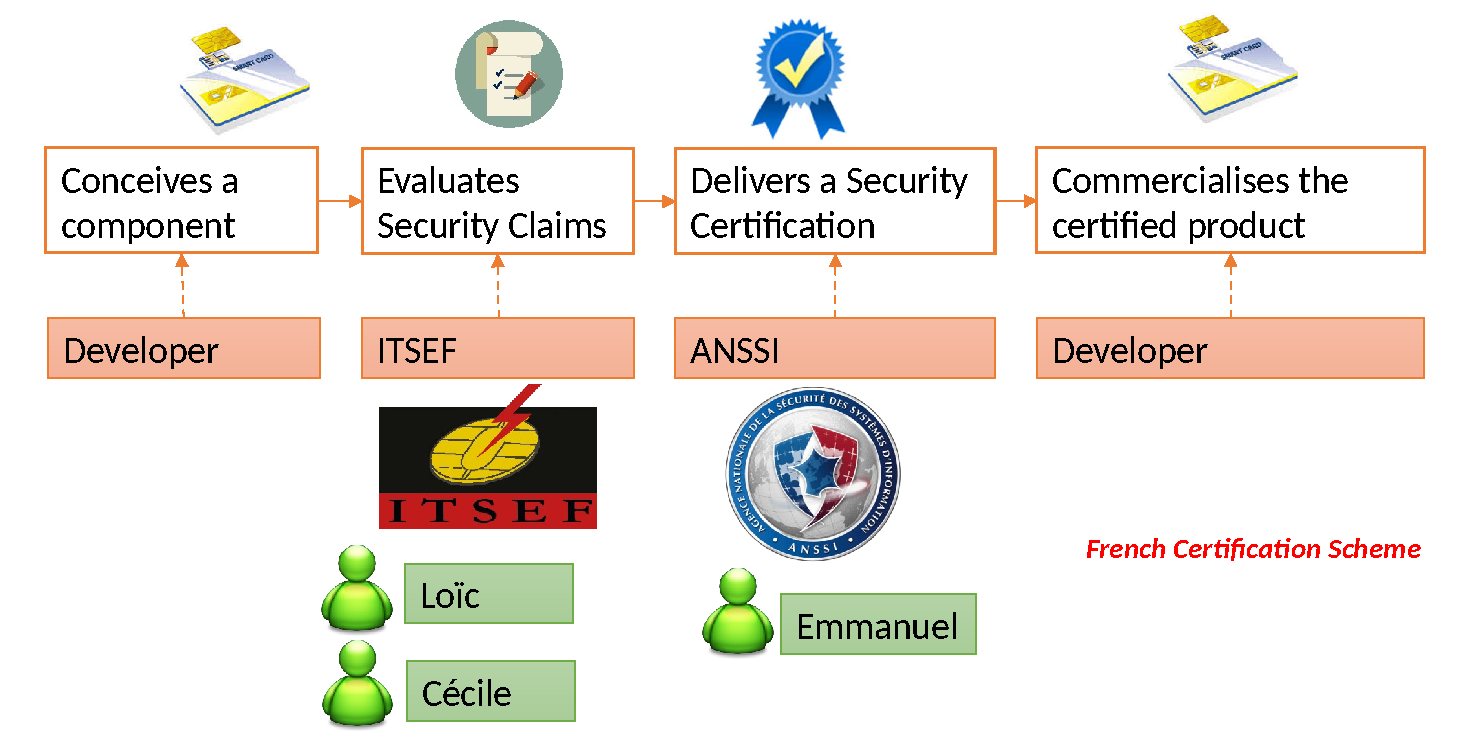
\includegraphics[width=\textwidth]{Figures/ITSEF_ANSSI_loic}
	\caption{The French certification scheme.
	Inspired from Cagli~\cite{cagli_these_2018}.}
	\label{fig:french_scheme}
\end{figure}

% Usual schemes
The most famous scheme is the \gls{cc} created in 1999, gathering several national certification bodies around the world.
The fact that those different certification bodies use the same scheme contributes to the standardization of the certification of security assessment.
Hereafter, we briefly present the different stakeholders of a certification scheme, depicted on \autoref{fig:french_scheme}.
\begin{itemize}
	\item \textbf{The Developers}
	conceive the product for which they ask a security certification.
	Asking a security certification is not mandatory, but often represents key stakes for the final product, \eg{} commercial advantage over a similar product.
	In the certification scheme, the product is referred as the \gls{toe}
	\item \textbf{The Evaluators}:
	When the certification query is claimed by the developer, the latter one ask an evaluation laboratory to assess the security of the \gls{toe}
	An evaluation laboratory is often referred under the name of \gls{itsef} -- \gls{cesti} in French.
	To evaluate the security of the \gls{toe} claimed by the developers, the \gls{itsef} verifies the expected functionalities, by inspecting not only the specifications of the \gls{toe}, the \gls{toe} as itself and -- depending on the required level of security -- the other components of the products which interact with it.
	Eventually, depending on the whole lifecycle of the \gls{toe}, some inspections on site -- \eg{} foundries -- may be done.
	If vulnerabilities are identified, the evaluator imagines threat scenarios by building attack paths, in order to assess the required means to succeed the attack, in terms of human, material and financial resources, or technical expertise.
	If need be, the evaluator realizes himself the attack -- or at least a part of it -- in order to verify the reliability of its assessment.
	Based on his investigations, the evaluator produces an \gls{etr}, sent to the developers and to the certification body.
	\item \textbf{The Certification Body}
	delivers the security certification, based on the \gls{etr} produced by the \gls{itsef}.
	Usually, the certification body is a governmental organization, such as the \gls{anssi} in France or the \gls{bsi} in Germany, but it can also be a private organization such as the \gls{emvco}.
	Sometimes if needed, the certification body can ask the \gls{itsef} for further investigation.
	Likewise, it can even verify that the evaluation has been correctly conducted by the \gls{itsef}, either by reproducing some parts of the evaluation on its own or by ordering audits into the evaluation laboratory. 
	The certificate is often made public to ensure not only the developers but also the final users about the claimed security of the \gls{toe}%
	\footnote{
		In France, security certifications are available on the \gls{anssi}'s website: \url{https://www.ssi.gouv.fr/entreprise/produits-certifies/}.
		An equivalent list of certification stamped by the \gls{bsi} is available at \url{https://www.bsi.bund.de/DE/Themen/ZertifizierungundAnerkennung/Produktzertifizierung/ZertifizierungnachTR/ZertifizierteProdukte/zertifiz_produkte.html?nn=6618104}
	}
\end{itemize}

\subsection{The Need of Constant Improvement of the State of the Art}
As a starting point of this section, it is interesting to more precisely define what the term ``\emph{security}'' means, and more particularly to point out the difference with the meaning of the term ``\emph{safety}'', despite their closeness.
% Def safety
\begin{quote}
	``The safety describes a machine designed to prevent inadvertent or hazardous operation''~\cite{mw:safety}, \ie{}\,``depending on the effect of \emph{unpredictable} and \emph{unanalyzable} forces in determining events''~\cite{mw:hazardous}.
\end{quote}
In other words, this definition assumes that an undesirable event mainly involves randomness.
% CSQ on safety
Assessing the safety of a device consists in verifying that the final user, is not likely to make -- unintentionnaly -- the device having a behavior not expected by its functional specifications. 

% Def security
Security is defined as 
\begin{quote}
	``to relieve from exposure to danger : act to make safe against \emph{adverse} contingencies''~\cite{mw:security}.
\end{quote}
% CSQ on security
Thus, assessing the security suggests to consider an \emph{adversarial} model threat: if there is a vulnerability in the device, one must assume that such an adversary -- \aka{} the \emph{attacker} -- will do all its possible to exploit it, provided it fits with the required means of this attack.
On the contrary, what is considered as a vulnerability in the \gls{toe} from a security point of view is not necessarily harmful from a safety point of view, as long as the probability to randomly encounter this vulnerability is sufficiently low.

Since the electronic devices embedding security functionalities are usually widely spread and are often used for critical tasks, such as telecommunications, banking transactions, \etc{} it is preferrable for the developer to consider an adversarial threat model, even if it requires to protect a device against potential attacks that are not likely to happen in real life.
Hence, one of the goals of developers and evaluators is to succeed in proving that a crypto-system is sound against \emph{any} attacker instantiating a given threat model.

At first sight, the latter task seems untractable, especially if there are infinite ways to instantiate an attacker from a threat model: it becomes impossible to test them all.
One way to circumvent this issue is to find a way to sort the different instances of a model threat according to their \emph{efficiency},%
\footnote{
	A formal definition of the term ``efficiency'' will be given in \autoref{sec:factors_attack_complex}.
}
in the sense that any attack being successful would necessarily imply that any more efficient attack would succeed.
Therefore, if the most efficient instance from a model threat does not succeed in breaking a target, one is guaranteed that any other attack within this threat model would fail too.

As a consequence, it is necessary for an evaluator to always reach the optimal attack, which consists in assessing the worst-case security, in order to provide strong guarantees about the security of the \gls{toe}
This requires an \gls{itsef} to always know the state-of-the-art attacks, and to be willing to always investigate how to push the limits of these attacks, in order to assess to what extent the security guarantees of a \gls{toe} may decrease through the time, as the \gls{sca} literature improves at the same time, making attacks of a given threat model more powerful.